\chapter{Understanding Links Using Nodes}







\section{Capture spatial non-stationarity (Proposed problem 1)}




\subsection{Dynamic spatial model}


We use various types of data to estimate the crime count in community area (CA) of Chicago. For each CA we have observations on crime count and demographics. For each pair of CAs we also have observations on the taxi flow and spatial distance. One straightforward method is to build a regression model from all the features we observed to the crime counts.

We have one interesting observations is that in the south and north part of Chicago, the significance of different features are different. Therefore, the idea is to learn a dynamic weights for different spatial region.



Suppose we have $n$ regions in total, $R = \{ r_1, r_2, \cdots, r_n \}$.
The following notations are used

\begin{table}[h]
\centering
\begin{tabular}{|l|r|}
\hline
crime count at $r_i$ & $y_i$ \\ \hline
demographics at $r_i$ & $\mathbf{d}_i$ \\ \hline
taxi flow between $r_i$ and $r_j$ & $f_{ij}$ \\ \hline
taxi flow weight matrix for $r_i$ & $\mathbf{f_i}$ \\ \hline
spatial weight matrix for $r_i$ & $\mathbf{g_i}$ \\ \hline
social flow lag variable for $r_i$ & $s_i = \mathbf{f}_i^T \mathbf{y}$ \\\hline
spatial flow lag variable for $r_i$ & $p_i = \mathbf{g}_i^T \mathbf{y}$ \\\hline
\end{tabular}
\caption{Symbols for the dynamic coefficient model.}
\end{table}


\subsubsection{Dynamic linear regression model}



For simplicity we use linear regression model
\[
y_i = \mathbf{w}_1^T \mathbf{d}_i + w_2 s_i + w_3 p_i + w_4,
\]
where $\{ w \}$ are the coefficients.

To simplify notations, we use $\mathbf{x}_i$ denote all the available predictors for region $r_i$,
\[
\mathbf{x}_i = [ \mathbf{d}_i, s_i, p_i, 1 ].
\]
Then the model becomes 
\[
y_i = \mathbf{w}^T \mathbf{x}_i.
\]



Now we use a dynamic model, where $\mathbf{w}$ is different for various regions.
This leads to 
\[
y_i  = \mathbf{w}_i^T \mathbf{x}_i.
\]


The problem with formulation is that there are too many parameters to learn. To address this issue, we use the constraint that \textbf{spatially adjacent regions share similar coefficients}.

We use $S_{ij}$ to denote the adjacency of $r_i$ and $r_j$. And the aforementioned constraint is formulated as
\[
\min \sum_{i,j} S_{ij} ||\mathbf{w}_i^T - \mathbf{w}_j^T||_2^2
\] The several choice of $S_{ij}$
\begin{itemize}
\item Binary indicator. $S_{ij} = 1$ if two regions are contiguous, otherwise $S_{ij} = 0$.
\item The reverse distance between $r_i$ and $r_j$. 
\end{itemize}

The overall objective is

\begin{equation}
\label{eq:obj}
\min_{\mathbf{W}}  \sum_i || y_i - \mathbf{w}_i^T \mathbf{x}_i ||_2^2 + \eta \sum_{i,j} S_{ij} ||\mathbf{w}_i^T - \mathbf{w}_j^T||_2^2 
+ \theta || \mathbf{W} ||_F^2
\end{equation}




\subsubsection{Optimization}


Rewrite the Frobenius norm in the last term
\[
|| \mathbf{W} ||_F^2 = \sum_i || \mathbf{w}_i - \mathbf{0}||_2^2.
\]


Therefore the Equation~\ref{eq:obj} is rewritten as
\begin{equation}
\label{eq:obj2}
\min_{\mathbf{W}}  \sum_i || y_i - \mathbf{w}_i^T \mathbf{x}_i ||_2^2 + \eta \sum_{i,j \in 0, \cdots, N} S_{ij} || \mathbf{w}_i - \mathbf{w}_j ||_2^2,
\end{equation}
where $\mathbf{w}_0 = \mathbf{0}$ and $S_{0i} = 1$ for $\forall i$.


To solve the objective in Equation~\ref{eq:obj2}, we use variable splitting. Namely, when optimizing for $\mathbf{w}_i$, we assume all other $\mathbf{w}_{j, j\neq i}$ are fixed. The sub-problem is
\begin{equation}
\label{eq:subobj}
\min_{\mathbf{w}_i}   ||y_i - \mathbf{w}_i^T \mathbf{x}_i ||_2^2 + \eta \sum_j S_{ij}|| \mathbf{w}_i - \mathbf{w}_j||_2^2.
\end{equation}



The update on $\mathbf{w}_i$ is
\[
\mathbf{w}_i = \min_{\mathbf{w}_i}   ||y_i - \mathbf{w}_i^T \mathbf{x}_i ||_2^2 + \eta \sum_j S_{ij} || \mathbf{w}_i - \mathbf{w}_j^{(t)} ||_2^2.
\]

The closed-form solution is

\begin{equation}
\mathbf{w}_i = (\mathbf{x}_i^T \mathbf{x}_i + \eta \sum_j S_{ij} \mathbf{I} )^{-1} (y_i \mathbf{x}_i + \eta \sum_j S_{ij} \mathbf{w}_j) 
\end{equation}


\subsubsection{Inference}

We use the \textbf{leave-one-out} setting to infer and evaluate the crime rate of new community area. 

Suppose the we want to estimate the crime rate $y_i$ of $CA_i$. During the training process, we hold everything about $CA_i$ out (including $y_i$, flow coming in and leaving from $CA_i$). Then training the model on $CA_j$, $\forall j \neq i$, which gives us $w_j$, $\forall j \neq i$. To infer the $y_i$, we need estimate the model coefficient $w_i$ first. Follow the same intuition that model on $CA_i$ is only similar to all its neighboring models, we have
\begin{equation}
\min_{\mathbf{w}_i} \sum_{j, \forall j \neq i} S_{ij} || \mathbf{w}_i - \mathbf{w}_j ||_2^2 + || \mathbf{w}_i ||_2^2
\end{equation}

After getting $\mathbf{w}_i$, we infer $y_i$ by
\begin{equation}
\hat{y}_i = \mathbf{w}_i^T * \mathbf{x}_i
\end{equation}



\section{Consider complicated interaction (Proposed problem 2)}


\subsection{Problem Formulation}

We want to predict the crime rate $y_i$ of each geographical grid (tract/community area) $g_i$. The available observations are demographics features $\x_i$ of each $g_i$ from census, and the interactions among grids. We denote the interactions as $\f_{ij}$ for grid pair $g_i, g_j$, and examples of such interactions are social flow and geospatial distance.

\subsection{Conditional random field model}
The first model comes to mind.

\subsubsection{Potential Function}
Each grid is a node, and its crime rate $y_i$ is the hidden variable that we want to estimate. Two kinds of fixed parameters are observed for each grid $g_i$. The first one is the demographic features $\x_i$. The second is the interactions among grids, such as social flow and geospatial distance, denoted by $\f{ij}$.

We use Conditional Random Field (CRF) shown in Figure~\ref{fig:crf} to model the dependency of nodal features. The learning goal is to estimate the conditional probability of $y$ given $\x$ and $\f$

\begin{equation}
	P(y |  \x, \f) 
\end{equation}


\begin{figure}[hb]
	\centering
	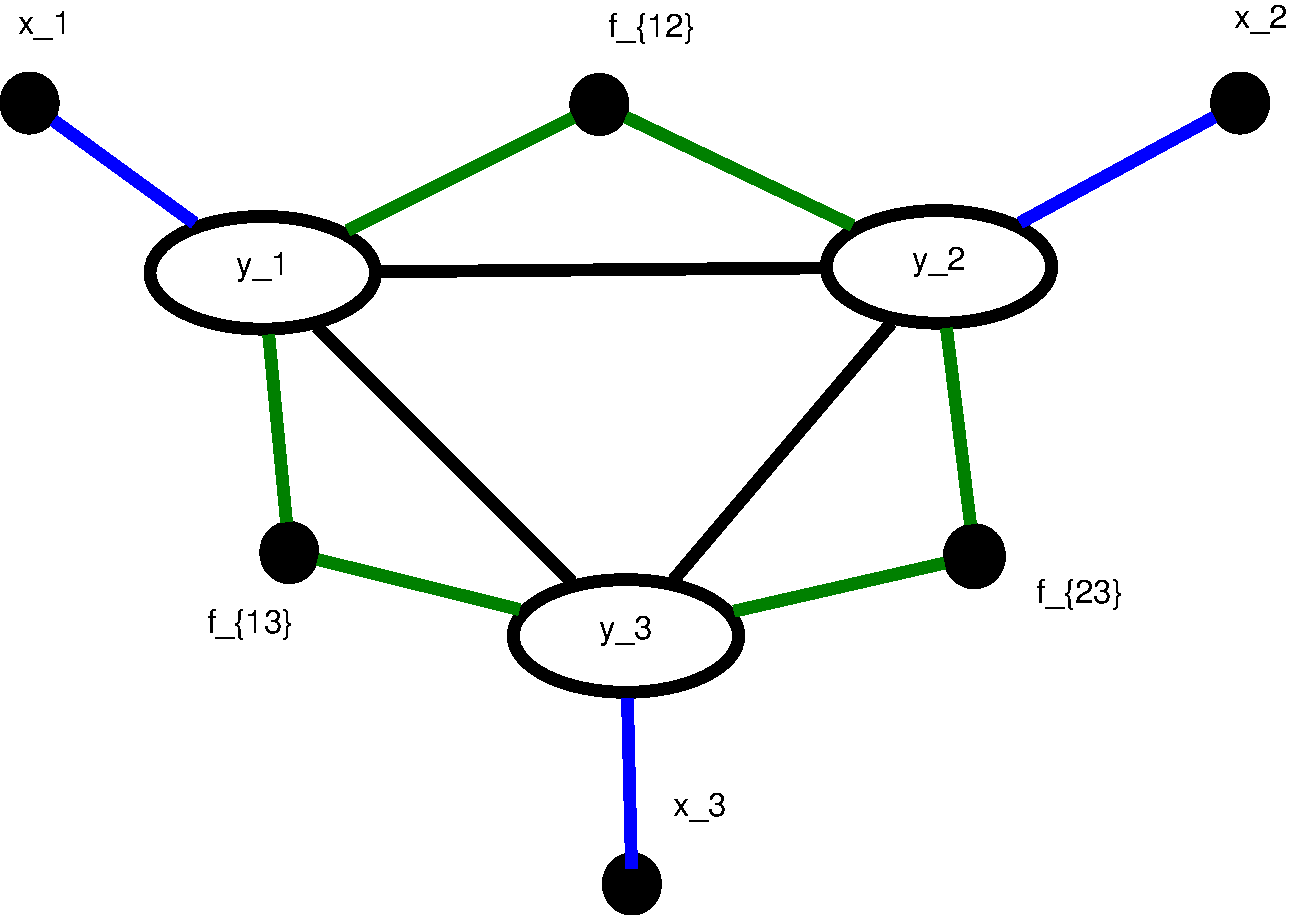
\includegraphics[width=0.5\textwidth]{fig/CRF-fig.pdf}
	\caption{The CRF model of the crime rate $y_i$ for each grid $g_i$.}
	\label{fig:crf}
\end{figure}



In the CRF model, we factorize the probability distribution of $y$ to a series of potential functions $\psi$ on the clique. 
\begin{equation}
	P(Y) = \frac{1}{Z} \prod_{ c \in C} \psi(c)
\end{equation}

Use $C_1$ to denote the set of cliques of size 1 with the form $\langle y_i \rangle$, and $C_2$ to denote size-2 clique. We define the potential function as follows:

\begin{align}
	\psi_{C_1} = &exp( - |y_i - \demow^T \cdot \x_i| )  \forall i \in [1, n], {g_i} \in C_1, \\
	\psi_{C_2} = & exp( - |y_i - y_j - \w^T \cdot \f_{i,j}| )  \forall i,j \in [1, n], {g_i, g_j} \in C_2, 
\end{align}
where $\demow$ and $\w$ are all positive coefficients.

The distribution of $Y$ is given by 
\begin{equation}
	P(Y) =  \frac{1}{Z} \left[ \prod_{i=1}^n \psi_{C_1}(y_i) \times \prod_{i=1}^n \prod_{j=i}^n \psi_{C_2}(y_i, y_j) \right]
\end{equation}
\begin{multline}
	P(Y) =  \frac{1}{Z} exp  \left( - \sum_{i=1}^n |y_i - \demow^T \cdot \x_i| \right. \\
          \left. - \sum_{i=1}^n\sum_{j=i}^n |y_i - y_j - \w^T \cdot \f_{i,j}| \right)
	\label{eq:PY}
\end{multline}


A large value of  potential function $\psi$ implies the high probability of $P(Y)$. The goal is to find a set of $Y$ maximizing $P(Y)$. 


\subsubsection{Inference}


\textbf{Estimate CRF Parameters}
\label{sec:estim}


We solve the Equation~(\ref{eq:PY}) by minimizing the negative log-likelihood function
\begin{multline}
\min_{\demow, \w} -\log P(Y|\demow, \w) = \min_{\demow, \w} \left[ \log Z + \sum_{i=1}^n |y_i - \demow^T \cdot \x_i| \right. \\
\left.  + \sum_{i=1}^n\sum_{j=i}^n |y_i - y_j - \w^T \cdot \f_{i,j}| \right]
\end{multline}

Use matrix form
\[
\min_{\demow, \w} ||X \demow - \y||_1 + ||F \cdot \w - \yp||_1,
\]
where $X$ is demographics matrix with $n$ rows, $\y$ is the $n$-dimension crime rate vector, $F$ is the pairwise features matrix with $(n^2+n)/2$  rows, and $\yp$ is the $(n^2+n)/2$-dimension pairwise crime rate difference vector $\{y_i- y_j\}$.

We can minimize separably.



\textbf{Minimize $\demow$}

\[ \min_{\demow} ||X \demow - \y||_1 \]

Take $X\demow - \y = \z$, and use ADMM.
\begin{multline}
 \min_{\z, \demow}  ||\z||_1 + \rho/2 ||\z - X\demow + \y||_2^2,\\
   s.t.\quad  \z - X\demow + \y = 0 
\end{multline}

\begin{multline}
L(\vec{\theta_1}, \z, \demow) = \max_{\vec\theta_1} \min_{\z, \demow} ||\z||_1 + \\
\rho/2 ||\z - X\demow + \y||_2^2  + \vec{\theta_1}( \z - X\demow + \y ) 
\end{multline}

\textbf{$\demow$ update}

\[ \demow^{k+1} \gets \argmin_{\demow}  \rho/2 ||\z^{k+1} - X\demow + \y + \vec{\theta_1}^{k+1}||_2^2 \]
Take derivative we have
\[ \frac{\partial}{\partial \demow} = \rho X^T(X\demow - \z^{k+1} - \y - \vec\theta_1^{k+1} ) \]
Make it $0$, $\demow^{k+1} = (X^TX)^{-1} X^T(\z^{k+1} + \y + \vec\theta_1^{k+1})$.

\textbf{$\z$ update}

\[ \z^{k+1} \gets \argmin_{\z}  ||\z||_1 + \rho/2 ||\z - X\demow^{k+1} + \y + \vec{\theta_1}^{k+1}||_2^2 \]
So, $\z^{k+1} = S_{1/\rho}(X\demow^{k+1} - \y - \vec\theta_1^{k+1})$.

\textbf{$\vec\theta_1$ update}

\[ \vec\theta_1^{k+1} = \vec\theta_1^{k} + \z^{k+1} - X\demow^{k+1} + \y \]



\textbf{Minimize $\w$}

\[ \min_{\w} ||F \cdot \w - \yp||_1 \]
It has exactly the same form as previously. Therefore,
\begin{multline}
L(\vec{\theta_2}, \z', \w) = \max_{\vec\theta_2} \min_{\z', \w}  ||\z'||_1 + \\
\rho/2 ||\z' - F\w + \yp||_2^2 + \vec{\theta_2}( \z' - F\w + \yp ) 
\end{multline}

\textbf{$\w$ update}
\[ \w^{k+1} = (F^TF)^{-1} F^T(\z^{'k+1} + \yp + \vec\theta_2^{k+1}) \]

\textbf{$\z'$ update}
\[ \z^{'k+1} = S_{1/\rho}(F\w^{k+1} - \yp - \vec\theta_2^{k+1}) \]

\textbf{$\vec\theta_1$ update}
\[ \vec\theta_2^{k+1} = \vec\theta_2^{k} + \z^{'k+1} - F\w^{k+1} + \yp \]



\textbf{Infer New $y_i$}

To infer new $y_i$, we want to maximize the following probability
\[ P(y_i | \x_i, F, \y, \demow, \w), \]
where $\demow$ and $\w$ are estimated using previous section, $\y$ denote the crime rates of other observed geographical units, and $F$ is the pairwise feature matrix.

Take negative log of the probability, we have 

\begin{align}
\min_{y_i} &  \left[ \log Z +  |y_i - \demow^T \cdot \x_i| + \sum_{j \neq i}^n |y_i - y_j - \w^T \cdot \f_{i,j}| \right] \nonumber \\
\min_{y_i} & \left[ |y_i - \demow^T \cdot \x_i| + \sum_{j \neq i}^n |y_i - y_j - \w^T \cdot \f_{i,j}| \right] 
\label{eq:inference}
\end{align}

In Equation~\ref{eq:inference}, we have $n+1$ $\ell_1$-norm terms, which have exactly the same form $|y_i - b_j|$. The objective becomes
\begin{equation}
  \min_{y_i} \sum_j^n |y_i - b_j|,
\label{eq:infy}
\end{equation}
where $b_1 = \demow^T \cdot \x_i$ and $b_j = y_{j-1} + \w^T\cdot \f_{i,j-1}$ for $j > 1$.

Notice that the optimal solution must take value on $\{b_j\}$. We solve this by sorting all the $b_j$ and then calculate the result segment by segment.




